%%%%%%%%%%%%%%%%%%%%%%%%%%%%%%%%%%%%%%%%%%%%%%%%%%%%%%%%%%%%%%%%%%%%%%%%%%%%%%%%
%2345678901234567890123456789012345678901234567890123456789012345678901234567890
%        1         2         3         4         5         6         7         8

\documentclass[letterpaper, 10 pt, conference]{ieeeconf}  % Comment this line out
                                                          % if you need a4paper
%\documentclass[a4paper, 10pt, conference]{ieeeconf}      % Use this line for a4
                                                          % paper
\usepackage{graphicx}
\IEEEoverridecommandlockouts                              % This command is only
                                                          % needed if you want to
                                                          % use the \thanks command
\overrideIEEEmargins
% See the \addtolength command later in the file to balance the column lengths
% on the last page of the document



% The following packages can be found on http:\\www.ctan.org
%\usepackage{graphics} % for pdf, bitmapped graphics files
%\usepackage{epsfig} % for postscript graphics files
%\usepackage{mathptmx} % assumes new font selection scheme installed
%\usepackage{times} % assumes new font selection scheme installed
%\usepackage{amsmath} % assumes amsmath package installed
%\usepackage{amssymb}  % assumes amsmath package installed

\title{\LARGE \bf
A Statistical Analysis of Cricket One Day Internationals
}

%\author{ \parbox{3 in}{\centering Huibert Kwakernaak*
%         \thanks{*Use the $\backslash$thanks command to put information here}\\
%         Faculty of Electrical Engineering, Mathematics and Computer Science\\
%         University of Twente\\
%         7500 AE Enschede, The Netherlands\\
%         {\tt\small h.kwakernaak@autsubmit.com}}
%         \hspace*{ 0.5 in}
%         \parbox{3 in}{ \centering Pradeep Misra**
%         \thanks{**The footnote marks may be inserted manually}\\
%        Department of Electrical Engineering \\
%         Wright State University\\
%         Dayton, OH 45435, USA\\
%         {\tt\small pmisra@cs.wright.edu}}
%}

\author{Nikhil Lohia, Arizona State University\\nlohia1@asu.edu, 1211168085}


\begin{document}



\maketitle
\thispagestyle{empty}
\pagestyle{empty}


%%%%%%%%%%%%%%%%%%%%%%%%%%%%%%%%%%%%%%%%%%%%%%%%%%%%%%%%%%%%%%%%%%%%%%%%%%%%%%%%


%%%%%%%%%%%%%%%%%%%%%%%%%%%%%%%%%%%%%%%%%%%%%%%%%%%%%%%%%%%%%%%%%%%%%%%%%%%%%%%%
\section{Introduction}

Cricket is an extremely popular game since last five centuries and played in countries all over the world. Being extremely fast paced and competitive it has been gaining audience steadily over time. Its ever increasing popularity has brought performance analysis to the team dressing room. There are several attributes which decide the outcome of a game; the team winning the toss, field conditions, the pitch and most importantly the performance of individual players. A game of cricket mainly has three aspects - batting, bowling and fielding. The team playing first sets a target and the other team bats next to chase it. If the second team is successful in chasing the target, they win the game else they lose. Thus, it is evident that batting statistics of a team really matters. It is essential for a team to score a high number of runs in the given number of balls.\\ 

\indent If we could somehow visualize the performance of players then the insights could help in assessing a game better. For instance, players can try to become technically better by observing their own performance, a team can plan a strategy in advance before facing it's opponent and thirdly the organizing committee can even decide which players to choose for the next game.\\

\indent But the bottleneck is that each game of generates a humongous amount of data and it is almost impossible to comprehend without some sort of visual representation. Thus, the project aims at creating a system with four interactive data visualizations which helps the user to explore and identify underlying trends of a team and players.\\

\section{System Goals and Scope}
\noindent The system serves two types of audience
\begin{itemize}
\item A sports journalist who wants to analyze a team's performance
\item A fan who wishers to discover the trends of his/her favorite team or player.
\end{itemize}
Keeping them in mind we decided upon two design principles
\begin{itemize}
\item The user should be able to select what he wants to see
\item Make the system interactive enough which forces the user to explore hidden insights from the data.
\end{itemize}
Some of the key insights that the audience might be interested in could be the player's contribution to team success, team vs team metrics and performance against different teams.\\
\noindent As per the guidelines of Kuchinsky et al. \cite{kentucky} multiple views are used when there is diversity in attributes and level of abstraction. In our cricket data we have a lot of information like player name, player country, home ground, played against etc. Therefore, a cricket game cannot be represented as a single visualization and it is essential to break the data into manageable chunks to bring out a correlation between them. The system should remain consistent even after having multiple views.

\section{System Overview}
The stacked area chart in itself and along with the other visualizations can be used effectively to identify key insights related to the performance of a team and its players.
\begin{figure}[!ht]
\centering
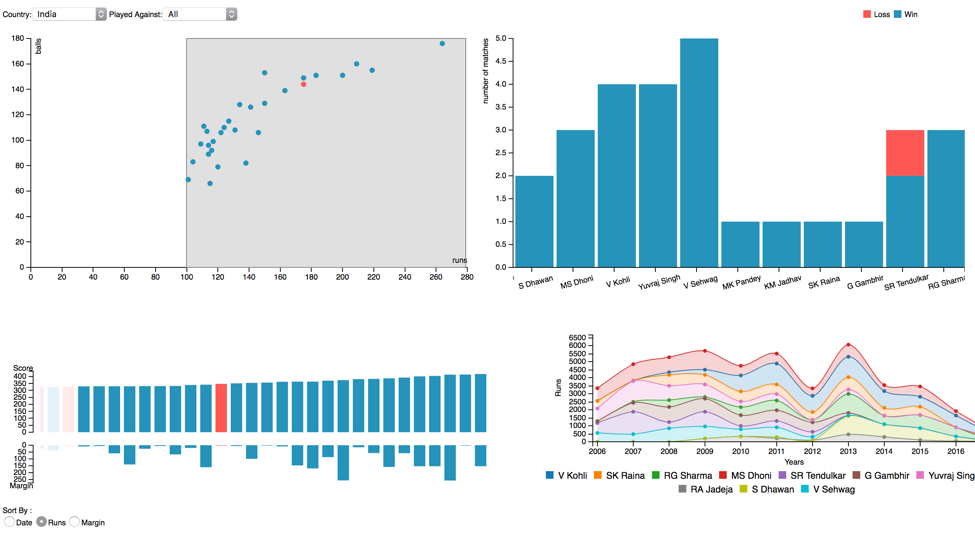
\includegraphics[width= 8.5cm]{case4.png}
\caption{System Overview}
\end{figure}
The system consists of four modules and we provide the user with two drop-down menus, that list the names of the various cricket playing nations. These drop downs provide an effective way of filtering the results based on a team and the opposition it has played against. Changing these values make an impact over the overall figures.

\section{Individual Contribution}
\subsection{Analytical Contribution} Identified the key parameters which could determine the outcome of the game and what is the relation between them. What would be the attributes of a good batsmen and a poor one? I also took a part in the idea to plot a bar chart with the brushing area selected in the scatter plot.

\subsection{Data Filtering}
After obtaining the data from Cricsheet\cite{cricsheet}, we were required to identify and extract the relevant values to our visualization. I extracted all these values and formed 3 tables which would be used in our visualization. The tables are then ingested into the system. The tables are stored as comma separated values as follows
\begin{itemize}
\item matchTable.csv
\begin{verbatim}
match_id,team_1,team_2,
team_1_runs,team_2_runs,
outcomeBy,outcomeByValue,winner,date
\end{verbatim}
\item performanceTable.csv
\begin{verbatim}
match_id,playerName,runsScored,
ballsFaced,team,result,opposition
\end{verbatim}
\item streamTable.csv
\begin{verbatim}
playerName,runsScored,date,
team,opposition
\end{verbatim}
\end{itemize}

\subsection{Rendering and Visualization}
One of the main insights of our project is analyzing a players performance over the years. It was my responsibility to visualize this information and I used the concept of stacked area chart. Stacked area graphs are useful for comparing multiple variables changing over an inter- val and discover trends across a wide range of groups. I used a spline-based area as it makes the graph look aesthetically pleasing. The years are presented on the X- Axis, whereas the Y-Axis shows the total number of runs scored.
\begin{figure}[!ht]
\centering
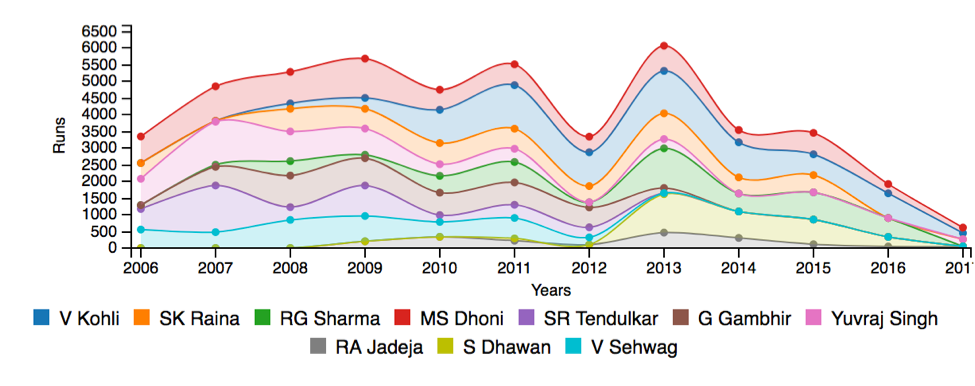
\includegraphics[width= 8.5cm]{india_case3.png}
\caption{Stacked area graph showing performance of Indian team}
\end{figure}
Stacked area chart is an extremely effective visualization in visualizing the performance of the team based on the sum of the number of runs, the players of the team, have been scoring each year. Each color in the graph represents a player and the width defines the number of runs scored by that specific player. The graph follows the Shneiderman’s mantra\cite{mantra} as it gives an overview of the team’s performance.\\
\noindent This visualization shows the trends of a team. Peaks mean a good performance and we can compare them with the actual events in timeline.
\noindent I also added interaction in the graph to see the individual contribution of each player at any time.

\subsection{Findings and Analysis:}
The stacked bar chart proves a lot of events that actually took place. India who were the winners of the International Cricket World Cup in the year 2011 and the winners of the ICC Champions trophy in 2013 were at the top of their performance in both those year.\\
\noindent Sri Lanka saw the retirement of 3 of its high scoring batsmen \textit{Jayawardene, Sangakara} and \textit{Dilshan} in the same year and maybe that is the reason their performance degraded all of a sudden.\\
\noindent By observing the player colors, we can also determine which players have been consistent over time. In the above example, we can see that \textit{Dravid} has been a consistent player over the years, while \textit{Yuvraj} started off as a hard hitter, phased out in the middle and regained his form later.


\section{Key Learnings}
\begin{itemize}
\item The amount of information that can be represent on a unit area of screen is very limited and with the increasing data it becomes harder to extract relevant insights from it.
\item A user should be given some of interaction in the visualization such that he is motivated to explore the insights on his own without getting confused.
\item A visualization should have the option to reconfigure on some of the variables which in turn shows hidden trends. In the project we have the option to sort the matches based on number of runs, the date played and the winning margin. Surprisingly, high number of runs resulted in winning a match.
\item The visualization should support change of parameters. The stacked area graph allows the user to toggle players. This shows how much impact that player makes on the team's overall performance.
\item Story telling in a visualization is extremely important. It should support the notion of chain and this can be done through texts, images and animations.
\item At the last, as stated by J. Mackinlay\cite{mackinlay} the goal is to create an insight and not pretty pictures. The visualization should be justified in every manner.
\item I also learned about C3, D3 and other related technologies which have been used in the system for data visualization.

\end{itemize}

\section{Team Members}
Aishwarya Pratap Singh, Ayushi Jain and Rahul Aakunuru

\section{Acknowledgement}
I am grateful to Prof. Ross Maciejewski for his constant encouragement and support towards the Project. At the end, I would humbly extend my thanks to all the team members whose constant hard-work and persistence brought a successful end to the project.

\begin{thebibliography}{99}

\bibitem{kentucky} Wang Baldonado, Michelle Q., Allison Woodruff, and Allan Kuchinsky. ``Guidelines for using multiple views in information visualization.'', \emph{Proceedings of the working conference on Advanced visual interfaces}. ACM, 2000.

\bibitem{mackinlay} Card, Stuart K., Jock D. Mackinlay, and Ben Shneiderman. ``Readings in information visualization: using vision to think''. \emph{Morgan Kaufmann}, 1999.

\bibitem{cricsheet} Cricsheet, ``http://cricsheet.org/downloads/odis\_male.zip''

\bibitem{mantra} Shneiderman, Ben. ``The eyes have it: A task by data type taxonomy for information visualizations.'' \emph{Visual Languages, 1996. Proceedings.}, IEEE Symposium on. IEEE, 1996.


\end{thebibliography}


\end{document}
